\section{Iterative schemes for highly forward-peaked scattering}
\subsection{Source Iteration and DSA}
\Cref{transport_operator} can be solved using the Source Iteration (SI)
method, which is a Richardson iteration, or a Krylov method. The Source
Iteration method at the $k^{th}$ iteration is given by:
\begin{equation}
\phi^{(k+1)} = \bs{DL}^{-1} \bs{M\Sigma}\phi^{(k)}+\bs{DL}^{-1}Q
\end{equation}
When the scattering ratio $c=\max_{l}\(\frac{\Sigma_{s,l}}{\Sigma_t}\)$ is close
to one, the spectral radius of SI can become arbitrary close to one and the
convergence becomes arbitrary slow. Since
most physical forward-peaked scattering produces $\Sigma_{s,0} >
\Sigma_{s,1}>\hdots$, the flat modes are the ones which should be accelerated
that is why the DSA scheme is used. The SI+DSA scheme is given by a transport sweep:
\begin{equation}
\phi^{(k+1/2)} = \bs{DL}^{-1}\bs{M\Sigma}\phi^{(k)} +\bs{DL}^{-1}Q,
\label{dsa_sweep}
\end{equation}
followed by a diffusion synthetic acceleration for the correction:
\begin{equation}
\delta \phi^{(k)} = \bs{\mc{T}}_0^{-1} \bs{R}_{n\rightarrow0}
\(\phi^{(k+1/2)}-\phi^{(k)}\),
\label{correction}
\end{equation}
yielding the next iterate for the flux moments:
\begin{equation}
\phi^{(k+1)} = \phi^{(k+1/2)} + \bs{P}_{0/1\rightarrow n} \delta \phi^{(k)}
\label{si_dsa_it}
\end{equation}
Finally, using \crefrange{dsa_sweep}{si_dsa_it}, we obtain:
\begin{equation}
\begin{split}
\phi^{(k+1)} =& \((\bs{I}+\bs{P}_{0/1\rightarrow n}\bs{\mc{T}}_0^{-1} \bs{R}_{n
\rightarrow 0}\bs{DL}^{-1} \bs{M\Sigma} - \bs{P}_{0/1\rightarrow n}
\bs{\mc{T}}_0^{-1} \bs{R}_{n\rightarrow 0}\) \phi^{(k)}\\
&+ (\bs{I} + \bs{P}_{0/1\rightarrow n}\bs{\mc{T}}_0^{-1} \bs{R}_{n\rightarrow
0}) \bs{DL}^{-1} Q
\end{split}
\label{dsa_it}
\end{equation}
where $\bs{\mc{T}}_0$ is the matrix associated to the DSA operator $\mc{T}_0$,
$\bs{R}_{n\rightarrow 0}$ is the restriction matrix of $\phi_n$ (all moments)
to $\phi_0$ (only $0^{th}$ moment) and $\bs{P}_{0/1\rightarrow n}$ the
projection matrix of $\phi_0$ or $\phi_1$, depending whether only the zeroth
or the zeroth and the first moment are accelerated, onto $\phi_n$. When only
the zeroth moment is accelerated, the scheme is always stable and the spectral
radius is max $\(\rho_{iso},\frac{\Sigma_{s,1}}{\Sigma_t}\)$ where
$\rho_{iso}$ is the spectral radius when the scattering is isotropic. In
multidimensional geometry, when both the zeroth and the first moments are
accelerated, the scheme is not always stable and the spectral radius is given
by $\(\rho_{iso},\frac{\Sigma_{s,1}}{\Sigma_{t}-\Sigma_{s,1}}\)$
\cite{multisweep}. For highly forward peaked scattering, accelerating the
zeroth moment is ineffective $\(\frac{\Sigma_{s,1}}{\Sigma_t}\rightarrow 1\)$,
whereas accelerating both moments can be unstable
$\(\frac{\Sigma_{s,1}}{\Sigma_t-\Sigma_{s,1}}>1\)$.

\section{Review of previous angular multigrid work}
\subsection{One dimensional geometry: the Morel and Manteuffel (MM) method}
As mentioned previously, only the zeroth and the first flux moments can be
accelerated with DSA. To accelerate higher moments, other methods have to be
used. Morel and Manteuffel proposed an angular multigrid method to accelerate
the SI calculation of the one-dimension $S_n$ equations with highly
anisotropic scattering \cite{multigrid_1d}. They use a variation of the
extended transport correction \cite{lathrop} to attenuate the ``upper half''
of the flux moments (higher frequencies) thanks to transport sweeps. The
``lower half'' of the flux moments (lower frequencies) is accelerated using
the $S_{n/2}$ equations. These $S_{n/2}$ equations are themselves accelerated
using $S_{n/4}$ equations. The order of the transport operator is divided by
two until the $S_4$ equations. The order of the transport operator is divided
by two until the $S_4$ level. At this point, the $P_1$ equations are used to
accelerate the $S_4$ equations. For the general where $n/2^i$ is odd, we need
to define:
\begin{equation}
Half(n) = \left\{
\begin{aligned}
&\frac{n}{2}, &\textrm{if }\frac{n}{2}\textrm{ is even}\\
&\frac{n}{2}+1, &\textrm{if }\frac{n}{2}\textrm{ is odd}
\end{aligned}
\right.
\end{equation}
Using this definition of ``Half'' to coarsen the angular grid, the sequence of
sweeps for an $S_{16}$ base level is $(S_{16}-S_8-S_4)$ and for a $S_{18}$
base level, the sequence is $(S_{18}-S_{10}-S_6-S_4)$. Morel and Manteuffel's
scheme works as follows:
\begin{enumerate}
\item Perform a transport sweep for the $S_n$ equations.
\item Perform a transport sweep for the $S_{n_2}$ equations with a $P_{n_2-1}$
expansions using the $S_n$ residual as the inhomogeneous source, where
$n_2=Half(n)$.
\item Continue coarsening the angular grid by a factor two (i.e., according to
the definition of ``Half'') until a sweep has been performed for the $S_4$
equations.
\item Solve the $P_1$ equations ($P1$ synthetic acceleration, $P1SA$) with a
$P_1$ expansion of the $S_4$ residual as the inhomogeneous source.
\item Add the Legendre moments of the $P_1$ solution to the Legendre moments
of the $S_4$ iterate to obtain the accelerated $S_4$ iterate.
\item Continue to add the corrections from each coarse grid to the finer grid
above to obtain the accelerated $S_n$ moments.
\end{enumerate}
Every time a transport sweep is performed, the optimal transport correction
needs to be used \cite{multigrid_1d}. For a $P_{n-1}$ expansion of the cross
sections, the corrected cross sections are given by:
\begin{equation}
\Sigma_{s,j}^* = \Sigma_{s,j} - \frac{\Sigma_{s,n/2}+\Sigma_{s,n-1}}{2}
\textrm{with }j-\{t\}\textrm{ or }\{s,l\}
\end{equation}
This correction is said to be optimal because for an infinite homogeneous
medium, it minimizes the ``high-frequency'' angular errors, the smoothing
factor being given by:
\begin{equation}
\rho_s =\max\(|\Sigma_{s,n/2}|/\Sigma_{s,0},|\Sigma_{s,n/2+1}|/\Sigma_{s,0},
\hdots,|\Sigma_{s,n-1}/\Sigma_{s,0}\)
\label{rho_s}
\end{equation}
To compare the effectiveness of the angular multigrid method with DSA,
Fokker-Planck scattering cross sections (\cref{sigma_m_sigma}) can be used. In
one dimension geometry, DSA becomes less efficient as $\Sigma_{s,l}$ $(0<l\leq
L)$ becomes closer to $\Sigma_{s,0}$. Therefore, in the limit as $L\rightarrow
\infty$, DSA no longer accelerates the convergence of SI for Fokker-Planck
scattering (the spectral radius tends to 1.0). However, the spectral radius of
the angular multigrid method has an upper bound of $0.6$ when $L\rightarrow
\infty$. It can be easily shown by using \cref{rho_s} and the fact that for
Fokker-Planck scattering cross sections the cross-section moments decrease
monotonically:
\begin{equation}
  \begin {split}
  \rho_s &= \frac{\Sigma_{s,N/2}^*}{\Sigma_{s,0}}\\
         &= \frac{3N-6}{5N-6}
  \end{split}
\end{equation}
which tends to 0.6 when $N$ goes to infinity.

The MM method converges in less iterations than DSA but it is important to
look at the cost of each MM iterations: one sweep in each $N$ directions + one
DSA iteration + one sweep in each ($\frac{N}{2}+\frac{N}{4}+\hdots$)
directions. Since $\frac{N}{2}+\frac{N}{4}+\hdots \leq N$, the cost of one MM 
iteration is less than: two sweeps in each $N$ directions + one DSA iteration.

\subsection{Multidimensional geometry: the Pautz-Adams-Morel (PAM) methods}
In the multidimensional case, DSA becomes unstable when both the zeroth and
the first flux moments are accelerated and $\frac{\Sigma_{s,1}}{\Sigma_t}\geq
0.5$, \cite{multisweep}. In \cite{multigrid_2d}, the authors modified the one
dimensional angular multigrid method by accelerating only the zeroth flux
moment with the DSA and by using $S_2$ as lowest transport sweep instead of
$S_4$. Even so, the proposed method (PAMNF, with ``NF'' for no-filtering) was
unstable and a filter was needed to stabilize the scheme (PAMF). Therefore,
the angular multigrid method was modified as follows \cite{multigrid_2d}:
\begin{enumerate}
\item Perform a transport sweep for the $S_n$ equations.
\item Perform a transport sweep for the $S_{n_2}$ equations with a $P_{n_2}$
for 2-D problem and a $P_{n_2+1}$ for 3-D problem expansion for the $S_n$
residual as the inhomogeneous source, where $n_2 = Half(n)$.
\item Continue coarsening the angular grid by a factor two (i.e., according to
the definition of ``Half'') until a sweep has been performed for the $S_2$
equations.
\item Solve the diffusion equation with a $P_0$ expansion for the $S_2$
residual as the inhomogeneous source.
\item Apply a diffusive filter to the corrections from steps 2 and 3 (without
this, the method is unstable).
\item Add the corrections from steps 4 and 5 to the Legendre moments of the
$S_n$ iterate to obtain the accelerated $S_n$ moments.
\end{enumerate}
The filter stabilizes the method which otherwise would diverge. Without the
filtering process, the low frequency are well attenuated but instabilities are
introduced in higher frequency modes. Filtering eliminates the high frequency
corrections which are well attenuated by SI alone but it keeps the low
frequency corrections. The filter is given by:
\begin{equation}
\(-\bn\cdot \frac{\beta_f}{3\Sigma_f}\bn + \Sigma_f\) f_{corr} = \Sigma_f
\(\phi_{n_2}+P_{n_4\rightarrow n_2}\phi_{n_4}+\hdots+P_{2\rightarrow
n_2}\phi_2\)
\end{equation}
where $\Sigma_f$ is the filter cross section and $\beta_f$ is the filter
tuning parameter. A Fourier analysis shows that given an input amplitude $A$,
the ``diffusively filtered'' amplitude is:
\begin{equation}
F=\frac{A}{1+\frac{\beta_f \lambda^2}{3\Sigma_f}}
\end{equation}
It is clear that the modes with large $|\lambda|$ (high frequencies) are
strongly attenuated while low-frequency are not. However, the filtering
process does not prevent the spectral radius from becoming arbitrary close to
1 when $L$ becomes large \cite{multigrid_2d}.

\section{Angular multigrid as preconditioner for Krylov Solvers}
In this research, we propose to abandon SI as the solver for the $S_n$
equations with highly-forward peaked scattering and to use a Krylov solver
instead. When using a Krylov solver, \cref{transport_operator} is rewritten as
follows:
\begin{equation}
(\bs{I}-\bs{DL}^{-1}\bs{M\Sigma})\phi = \bs{DL}^{-1}Q
\label{krylov_transport_operator}
\end{equation}
\Cref{krylov_transport_operator} is \cref{transport_operator} preconditioned
by $\bs{DL}^{-1}$ (transport sweep preconditioning). DSA can also help to
speed up the convergence of the Krylov solver and the DSA-preconditioned
system of equations solved with a Krylov method is:
\begin{equation}
\begin{split}
&\((\bs{I} + \bs{P}_{0/1\rightarrow n} \bs{\mc{T}}_0^{-1} \bs{R}_{n\rightarrow
0})(\bs{I}-\bs{DL}^{-1}\bs{M\Sigma})\) \phi=\\
&(\bs{I}+\bs{P}_{0/1\rightarrow n} \bs{\mc{T}}_0^{-1} \bs{R}_{n\rightarrow 0})
\bs{DL}^{-1} Q
\end{split}
\end{equation}
The angular multigrid scheme can also be recast to be used by a Krylov
solver. Here, we have chosen the recast the PAM method without filtering
(PAMNF) as a preconditioner for a Krylov solver. The successive corrections of
the angular multigrid acceleration form now different stages of a
preconditioner used in the Krylov solver. Two variations of the PAMNF
preconditioner will be tested:
\begin{itemize}
\item the coarsest level is DSA (ANMG-DSA) (with the coarsest $S_n$ level
being $S_2$).
\item the coarsest level is $P1SA$ (ANMG-P1SA) (with the coarsest $S_n$ level
being $S_4$).
\end{itemize}
First, we present the angular multigrid using DSA and then, the angular
multigrid using $P1SA$. Later, these two versions are compared.
\subsection{ANMG-DSA}
Using a method similar to the one we used to write the equation for the
preconditioned Krylov solver, we recast the PAMNF for SI as a preconditioner
for a Krylov solver. First, we write the SI sweep equation, the successive
corrections and the new iterate built from the sweep values plus all the
successive corrections:
\begin{align}
& \phi_n^{(k+1/2)} = \bs{D}_n\bs{L}_n^{-1}\bs{M}_n\bs{\Sigma}_n\phi_n^{(k)} +
\bs{D}_n \bs{L}_n^{-1} Q\\
& \delta \phi_{n_2}^{(k)} = \bs{D}_n\bs{L}_{n_2}^{-1} \bs{M}_{n_2}
\bs{\Sigma}_{n_2} \bs{R}_{n\rightarrow n_2}
\(\phi_n^{(k+1/2)}-\phi_n^{(k)}\)\\
& \hdots\\
& \delta \phi_2^{(k)} = \bs{D}_2 \bs{L}_2^{-1} \bs{M}_2 \bs{\Sigma}_2
\bs{R}_{4\rightarrow 2}\delta \phi_4\\
& \delta \phi_0^{(k)} = \bs{\mc{T}}_0^{-1} \bs{R}_{2\rightarrow 0}\delta
\phi_2^{(k)}\\
& \phi_n^{(k+1)} = \phi_n^{(k+1/2)} + \bs{P}_{n_2\rightarrow n} \delta
\phi_{n_2}^{(k)} + \hdots + \bs{P}_{2\rightarrow n} \delta \phi_2^{(k)} +
\bs{P}_{0\rightarrow n} \delta \phi_0^{(k)} \label{mom_update}
\end{align}
Now, all the corrections $\delta \phi_0^{(k)}$ through $\delta \phi_{n_2}^{k}$
are substituted into the moment update equation, \cref{mom_update}, yielding:
\begin{equation}
\begin{split}
\phi_n^{(k+1)} =& \bs{T}_n \phi_n^{(k)} + \bs{D}_n \bs{L}_n^{-1} Q +
\bs{P}_{n_2\rightarrow n}\(\bs{T}_{n_2}\bs{R}_{n\rightarrow n_2}
\(\phi_n^{(k+1/2)}-\phi_n^{(k)}\)\)+\hdots\\
&+\bs{P}_{2\rightarrow n} \bs{T}_2\bs{R}_{4\rightarrow 2} \delta \phi_4^{(k)}
+ \bs{P}_{0\rightarrow n} \bs{\mc{T}}_0^{-1} \bs{R}_{2\rightarrow 0} \delta
\phi_2^{(k)}\\
=& \bs{T}_n\phi_n^{(k)} + \bs{D}_n \bs{L}_n^{-1} Q + \bs{P}_{n_2\rightarrow n}
\(\bs{T}_{n_2} \bs{R}_{n\rightarrow n_2} \(\bs{T}_n \phi_n^{(k)} +\bs{D}_n
\bs{L}_n^{-1} Q -\phi_n^{(k)}\)\)\\
&+\hdots+\bs{P}_{2\rightarrow n} \bs{T}_2 \bs{R}_{4\rightarrow 2}\( \bs{T}_4
\bs{R}_{8\rightarrow 4} \(\hdots\(\bs{T}_n \phi_n^{(k)} + \bs{D}_n
\bs{L}_n^{-1} Q -\phi_n^{(k)}\)\)\)\\
&+ \bs{P}_{0\rightarrow n} \bs{\mc{T}}_0^{-1} \bs{R}_{2\rightarrow 0}
\(\bs{T}_2 \bs{R}_{4\rightarrow 2}\(\hdots\( \bs{T}_N\phi_n^{(k)} + \bs{D}_n
\bs{L}_n^{-1}Q -\phi_n^{(k)}\)\)\)\\
=& \( \bs{T}_n + \bs{P}_{n_2\rightarrow n} \bs{T}_{n_2} \bs{R}_{n\rightarrow
n_2} (\bs{T}_n -\bs{I}) + \hdots + \bs{P}_{2\rightarrow n} \bs{T}_2
\bs{R}_{4\rightarrow 2} \(\bs{T}_4 \bs{R}_{8\rightarrow
4}\(\hdots\(\bs{T}_n-\bs{I}\)\)\)\right.\\
&\left.+\bs{P}_{0\rightarrow n}\bs{\mc{T}}_0^{-1} \bs{R}_{2\rightarrow 0}
\bs{R}_{2\rightarrow 0} \(\bs{T}_2 \bs{R}_{4\rightarrow
2}\(\hdots\(\bs{T}_n-\bs{I}\)\)\)\) \phi_n^{(k)} +
\(bs{I}+\bs{P}_{n_2\rightarrow n}\bs{T}_{n_2} \bs{R}_{n\rightarrow n_2}+
\hdots +\right.\\
&\bs{P}_{2\rightarrow n} \bs{T}_2 \bs{R}_{4\rightarrow 2} \(\bs{T}_4
\bs{R}_{8\rightarrow 4}\(\hdots \(\bs{T}_{n_2} \bs{R}_{n\rightarrow
n_2}\)\)\)+\\
&\left. \bs{P}_{0\rightarrow n} \bs{\mc{T}}_0^{-1} \bs{R}_{2\rightarrow 0}
\(\bs{T}_2 \bs{R}_{4\rightarrow 2}\(\hdots\(\bs{T}_{n_2} \bs{R}_{n\rightarrow
n_2}\)\)\)\) \bs{D}_n \bs{L}^{-1} Q
\end{split}
\end{equation}
where we defined $\bs{T}_n = \bs{D}_n \bs{L}_n^{-1} \bs{M}_n \bs{\Sigma}_n$
(the subscript $n$ denotes the $S_n$ level). Finally, the linear system to be
solved is given by:
\begin{align}
  &\(\bs{I}-\bs{T}_n\) \bs{P}^{MG/DSA} \xi_n = \bs{D}_n \bs{L}_n^{-1} Q
  \label{p_mg_dsa_1}\\
  &\bs{P}^{MG/DSA} \phi_n = \xi_n \label{p_mg_dsa_2}
\end{align}
where the multigrid preconditioner $\bs{P}^{MG/DSA}$ is given by:
\begin{equation}
\begin{split}
  &\bs{P}^{MG/DSA} =\\
&\(\bs{I}+\bs{P}_{n_2\rightarrow n} \bs{T}_{n_2}
\(\bs{I}+\bs{P}_{n_4\rightarrow n_2}
\bs{T}_{n_4}\(\hdots\(\bs{I}+\bs{P}_{0\rightarrow 2}
\bs{\mc{T}}_0^{-1}\bs{R}_{2\rightarrow 0}\)\hdots\)\bs{R}_{n_2\rightarrow
n_4}\) \bs{R}_{n\rightarrow n_2}\)
\end{split}
\end{equation}
At this point, it is necessary to choose a DSA for implementation. Various DSA
schemes have been reviewed in \cite{dsa_ref,multisweep,consistent_p1,larsen_91,
wareing,trans_87}. We have chosen to employ the Modified Interior Penalty
(MIP) DSA scheme developed by Wang and Ragusa \cite{mip} (see next Chapter). 
The MIP-DSA scheme is based on a discretization of the diffusion equation rather 
than the $P1$ equations. More specifically, MIP uses a bilinear \emph{discontinuous} 
trial space, which is the same trial space as the one used for the $S_n$ transport
equations. However, the MIP equations are not fully consistent with the
bilinear-discontinuous spatial discretization of the transport equation. Full
consistency requires discretization of the $P1$ equations. The consistency
discretized $P1$ equations are of a non-symmetric mixed form. The MIP-based
DSA algorithm is always stable for isotropic scattering and the MIP diffusion
matrix is symmetric positive definite (SPD), which makes it much easier to
invert than the mixed $P1SA$ equation. For instance, one can use a conjugate
gradient technique, preconditioned with SSOR to solve the MIP equation.

\subsection{ANMG-P1SA}   
Using $S_4$ as the lowest $S_n$ order followed by a $P1SA$ acceleration
(instead $S_2$ followed by DSA) in \cref{p_mg_dsa_1,p_mg_dsa_2} yields the 
following linear system:
\begin{align}
  &\(\bs{I}-\bs{T}_n\)\bs{P}^{MG/P1SA} \xi_n = \bs{D}_n\bs{L}_n^{-1} Q\\
  & \bs{P}^{MG/P1SA} \phi_n = \xi_n
\end{align}
where the multigrid preconditioner $P^{MG/P1SA}$ is now given by:
\begin{equation}
\begin{split}
&P^{MG/P1SA} =\\
&\(\bs{I}+\bs{P}_{n_2\rightarrow n} \bs{T}_{n_2}
\(\bs{I}+\bs{P}_{n_4\rightarrow n_2}
\bs{T}_{n_4}\(\hdots\(\bs{I}+\bs{P}_{1\rightarrow 4}\bs{\mc{T}}_1^{-1}
\bs{R}_{4\rightarrow 1}\)\hdots\)\bs{R}_{n_2\rightarrow n_4}\)
\bs{R}_{n\rightarrow n_2}\) 
\end{split}
\end{equation}
where $\bs{\mc{T}}_1$ is the matrix associated to the $P1SA$ operator
$\mc{T}_1$ operator. The $P1SA$ discretization used here is the $P1C$ method,
defined in \cite{yaqiPhD,P1C_MC2009}. This $P1SA$ preconditioner is positive
definite (PD), but not symmetric. In principle, the analytic $P1$ equations
can be put in a second-order diffusion form and discretized using the MIP
approach. However, the first moments of the angular flux will be treated wit
less accuracy than the zeroth moment, which is undesirable.

\section{Eigenspectrum comparisons}
In this section, we compare the eigenvalue spectrum for a given model problem.
This is instructive because the convergence of GMRES is proportional to the
relative radii of the eigenvalue clusters and/or the maximal distance between
two clusters; furthermore, the eigenvalues close to zero are considered as
outliers that are processed one at a time and increase the asymptotic error
constant \cite{campbell}.  We use a $S_8$ Gauss-Legendre-Chebyshev Galerkin
triangular quadrature. The domain, a 5$cm-$side square uniformly discretized
using a 25 cells, is homogeneous. Fokker-Planck cross sections, with
$\alpha=1$ and $L=8$, are employed. For the spatial discretization, BiLinear
Discontinuous (BLD) finite elements are used (see next Chapter). $\Sigma_t$ 
is chosen to be equal to $\Sigma_{s,0}$. Figs. \ref{eig_sweep}-\ref{eig_anmg} 
show the eigenvalue spectrum for sweep preconditioning (Fig. \ref{eig_sweep}), 
DSA preconditioning (Fig. \ref{eig_dsa}), and angular multigrid preconditioning
(Fig. \ref{eig_anmg}). The eigenvalues were obtained using implicit QR
decomposition \cite{implicitQR}. Even though the global matrices are never
formed in transport solution techniques, we constructed them here for the
purposes of the eigenspectrum analysis (specifically, the $j^{th}$ column of
any matrix $A$ is obtained by multiplying it by the canonical basis vector
$e_j$).
\begin{figure}[H]
  \centering
  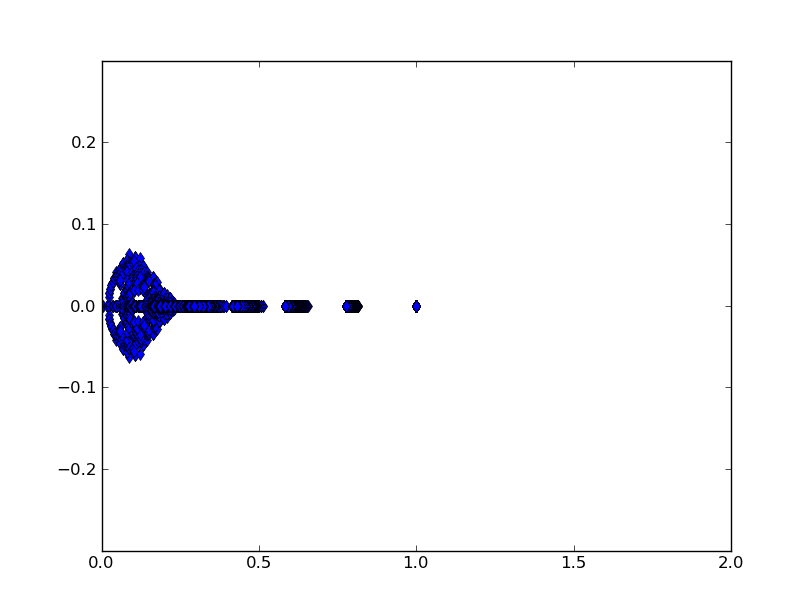
\includegraphics[width=0.5\textwidth]{./Anmg/s8_5_5}
  \caption{Eigenspectrum of the sweep preconditioned system}
  \label{eig_sweep}
\end{figure}
\begin{figure}[H]
  \centering
  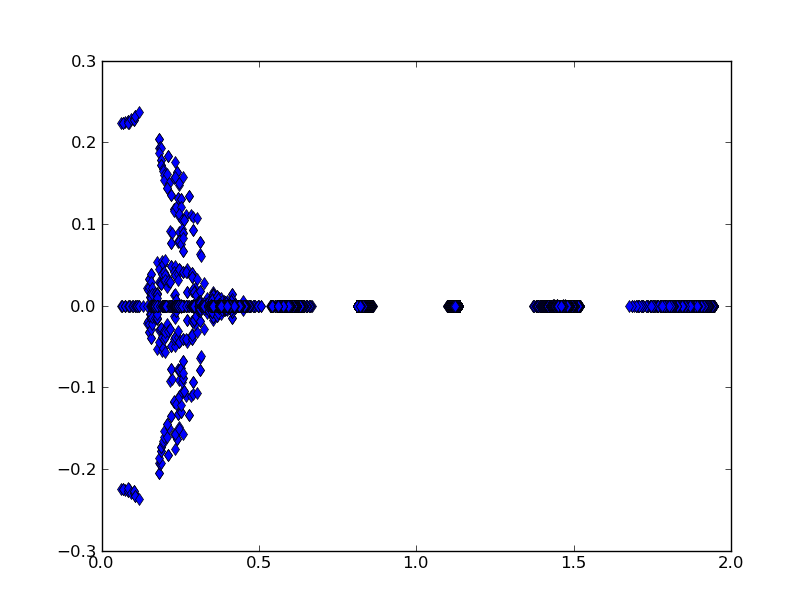
\includegraphics[width=0.5\textwidth]{./Anmg/d_s8_5_5}
  \caption{Eigenspectrum of the DSA preconditioned system}
  \label{eig_dsa}
\end{figure}
\begin{figure}[H]
  \centering
  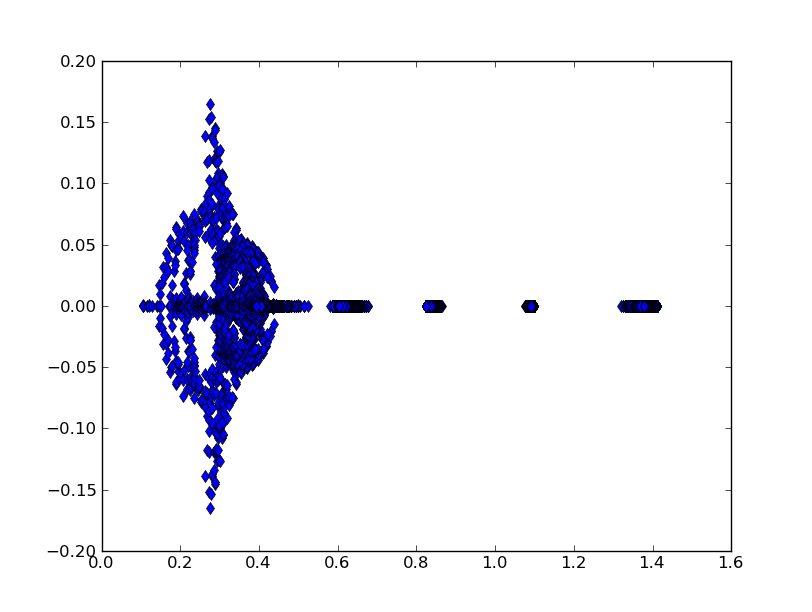
\includegraphics[width=0.5\textwidth]{./Anmg/p_s8_5_5}
  \caption{Eigenspectrum of the ANMG (DSA variant) preconditioned system}
  \label{eig_anmg}
\end{figure}
On these figures, we can note that sweep preconditioning is not effective as
many eigenvalues are located near zero. DSA moves the eigenvalues away from
zero. This explains the faster convergence of GMRES with DSA preconditioning
compared to sweep preconditioning. ANMG moves the eigenvalues even further
aways from zero than DSA and clusters them more compared to DSA. It is obvious
from these figures that ANMG preconditioning should converge much faster than
DSA preconditioning.

